\section{DDoS Dissector}
\label{sec:ddos_dissector}
%about fingerprint: concepts \& context}

A DDoS attack is composed of one or more single vector attacks. All single vectors of a DDoS attack are linked to one multivector key.

There are several words used by the academic and security community for defining DDoS attack fingerprint. The words are DDoS `characteristics', `fingerprint', `profile', `pattern', `signature', and `rule'. Oxford dictionary defines these words as the following.

\begin{itemize}
	\item \textbf{characteristics}: ``a feature or quality belonging typically to a person, place, or thing and serving to identify them'';
	\item \textbf{fingerprint}: ``a distinctive identifying characteristic'';
	\item \textbf{profile}: ``a graphical or other representation of information relating to particular characteristics of something, recorded in quantified form'';
	\item \textbf{pattern}: ``a regular and intelligible form or sequence discernible in the way in which something happens or is done'';
	\item \textbf{signature}: ``a distinctive pattern, product, or characteristic by which someone or something can be identified'';
	\item \textbf{rule}: ``a principle that operates within a particular sphere of knowledge, describing or prescribing what is possible or allowable'';
\end{itemize}

our definition  

Definition 2: DDoS fingerprint is the smallest set of features that summarizes the main characteristics of each attack vector in a DDoS attack, extracted from a network measurement of the attack.

Definition 3: Enriched version of the DDoS fingerprint may contain additional information generated by post-processing of the filtered and anonymized network measurement of the attack. Examples: (1) autonomous system of the source IP addresses; (2) geolocation of the source IP addresses; eventually (3) indication of spoofed IP addresses; and (4) open ports of source IP addresses closer to the moment of the attack.


\begin{figure}
	\centering
	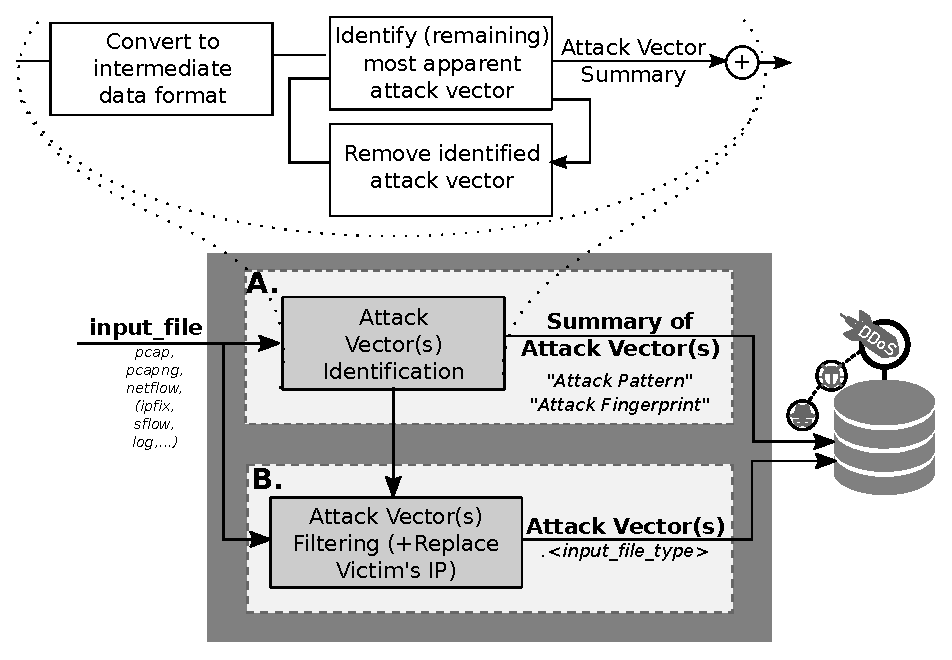
\includegraphics[width=0.5\textwidth]{{figs/ddos_fingerprinting.eps}}
	\caption{A picture of a gull.}
\end{figure}







 
